\documentclass[11pt]{article}
\usepackage[margin=1in]{geometry}
\usepackage{amsmath,amssymb,booktabs,graphicx,setspace,caption,hyperref}
\usepackage[T1]{fontenc}
\usepackage{mathpazo}
\setlength{\parindent}{0pt}
\setlength{\parskip}{0.6em}
\captionsetup{font=small,skip=6pt}
\title{Panel MS-AR(1): common trend, random intercepts, catch-up\\[0.4em]\large Seasonally adjusted real GDP per worker (period-average USD)}
\author{}
\date{}
\begin{document}
\maketitle
\section{Model}
Joint panel Markov-switching AR(1) around a \emph{linear} trend, with three regimes. The pooled and random-effects specifications are
\begin{align}
y_{it} &= a_i + g\, t + z_{it}, \\
z_{i,t+1} &= \bigl(1-\rho(s_{it})\bigr)\mu(s_{it}) + \rho(s_{it})\, z_{it} + \sigma(s_{it})\,\varepsilon_{it}, \\
s_{i,t+1} &\sim \Pi(\,\cdot\mid s_{it}).
\end{align}
In the pooled specification $a_i\equiv a$. In the random-effects specification $a_i\sim\mathcal{N}(\alpha,\omega^2)$; $\alpha$ and $\omega$ are estimated by maximum likelihood, integrating each country's Hamilton-filter likelihood by 11-point Gauss--Hermite quadrature. Cycles then use the posterior mean of $a_i$. Specifications 3 and 4 keep a permanent random intercept and add a decaying entry gap
\begin{align}
y_{it} &= a_i + g\, t + b_i\,\lambda^{t-T_{i0}} + z_{it}, \\
a_i &\sim \mathcal{N}(\alpha,\omega^2),\qquad b_i \sim \mathcal{N}(0,\omega_b^2) \ \text{independent}.
\end{align}
$T_{i0}$ is country $i$'s first observation. Spec 3 holds $\lambda=0.98$ (Barro 2\% per year). Spec 4 estimates $\lambda$ in $(0,0.985)$. The two random effects are integrated by $7\times 7$ Gauss--Hermite quadrature. The outcome is log seasonally adjusted real GDP per worker (period-average USD) from the 2026-09-17 quarterly panel. Calendar time is taken from the period stamp $t$ (year-fraction). $g$ is per year and common. Latent paths $s_{it}$ are country-specific. The regime dated $t$ governs the transition from $z_t$ to $z_{t+1}$. $\sigma$ and $\rho$ switch with the regime. The median $\mu$ is pinned at 0. $|\rho|<0.99$.
Standard errors (in parentheses) are delta-method from a numerical Hessian on shared parameters. $\pi$ is the ergodic distribution of $\Pi$. $E[z]$ is the long-run mean of the cycle implied by $\mu$, $\rho$, and $\Pi$.
\clearpage
\section{Common intercept and linear trend}
2026-09-17 SA panel, full sample: log real GDP per worker. 74 countries, 8670 observations, 1950-Q1--2026-Q2. Fitted countries: 74. Observations: 8670. Log-likelihood: 22607.90. Ergodic mean of the cycle $E[z]=0.7539$ (0.0689).
Common intercept $a=-6.0145$ (0.0592). Common slope $g=0.0079$ (0.0005).
\begin{table}[h]
\centering
\caption{Regime AR(1), transition matrix, and ergodic $\pi$. Columns are regimes.}
\begin{tabular}{lccc}
\toprule
 & (0) & (1) & (2) \\
\midrule
$\mu$ & -0.2212 & 0.0000 & 1.7476 \\
 & (0.0943) & --- & (0.0464) \\ \addlinespace
$\sigma$ & 0.0695 & 0.0161 & 0.0090 \\
 & (0.0019) & (0.0004) & (0.0002) \\ \addlinespace
$\rho$ & 0.9900 & 0.9900 & 0.9900 \\
 & (0.0000) & (0.0000) & (0.0000) \\ \addlinespace
$\Pi_{0\cdot}$ & 0.7511 & 0.1700 & 0.0789 \\
 & (0.0229) & (0.0206) & (0.0115) \\ \addlinespace
$\Pi_{1\cdot}$ & 0.0610 & 0.9337 & 0.0053 \\
 & (0.0063) & (0.0064) & (0.0022) \\ \addlinespace
$\Pi_{2\cdot}$ & 0.0279 & 0.0029 & 0.9692 \\
 & (0.0035) & (0.0016) & (0.0034) \\ \addlinespace
$\pi$ & 0.1487 & 0.4010 & 0.4502 \\
 & (0.0120) & (0.0301) & (0.0318) \\ \addlinespace
\bottomrule
\end{tabular}
\end{table}
\begin{figure}[h]
\centering

\includegraphics[width=0.75\textwidth]{figs/cycle_common_ag.pdf}
\caption{Country cycles after removing the linear trend.}
\end{figure}
\clearpage
\section{Random-effects intercepts, common linear trend}
2026-09-17 SA panel, full sample: log real GDP per worker. 74 countries, 8670 observations, 1950-Q1--2026-Q2. Fitted countries: 74. Observations: 8670. Log-likelihood: 23465.89. Ergodic mean of the cycle $E[z]=0.0559$ (0.0268).
Random intercepts $a_i\sim N(\alpha,\omega^2)$ with $\alpha=-5.9377$ (0.0424), $\omega=0.5121$ (0.0061). Posterior-mean $a_i$: mean -5.536, min -7.953, max -3.922. Common slope $g=0.0086$ (0.0005).
\begin{table}[h]
\centering
\caption{Regime AR(1), transition matrix, and ergodic $\pi$. Columns are regimes.}
\begin{tabular}{lccc}
\toprule
 & (0) & (1) & (2) \\
\midrule
$\mu$ & -0.8646 & 0.0000 & 0.2813 \\
 & (0.1094) & --- & (0.0354) \\ \addlinespace
$\sigma$ & 0.0750 & 0.0188 & 0.0070 \\
 & (0.0026) & (0.0005) & (0.0001) \\ \addlinespace
$\rho$ & 0.9899 & 0.9899 & 0.9898 \\
 & (0.0004) & (0.0001) & (0.0002) \\ \addlinespace
$\Pi_{0\cdot}$ & 0.7023 & 0.2780 & 0.0197 \\
 & (0.0319) & (0.0326) & (0.0091) \\ \addlinespace
$\Pi_{1\cdot}$ & 0.0580 & 0.8821 & 0.0599 \\
 & (0.0072) & (0.0103) & (0.0071) \\ \addlinespace
$\Pi_{2\cdot}$ & 0.0081 & 0.0474 & 0.9445 \\
 & (0.0029) & (0.0062) & (0.0055) \\ \addlinespace
$\pi$ & 0.0949 & 0.4190 & 0.4861 \\
 & (0.0098) & (0.0211) & (0.0247) \\ \addlinespace
\bottomrule
\end{tabular}
\end{table}
\begin{figure}[h]
\centering

\includegraphics[width=0.75\textwidth]{figs/cycle_re_ai.pdf}
\caption{Country cycles after removing the linear trend.}
\end{figure}
\clearpage
\section{RE intercepts plus catch-up, lambda fixed at Barro 0.98}
2026-09-17 SA panel, full sample: log real GDP per worker. 74 countries, 8670 observations, 1950-Q1--2026-Q2. Fitted countries: 74. Observations: 8670. Log-likelihood: 23563.79. Ergodic mean of the cycle $E[z]=0.0601$ (0.0275).
Permanent RE intercepts and catch-up $y_{it}=a_i + g t + b_i\lambda^{t-T_{i0}}+z_{it}$ with $\alpha=-5.7753$ (0.0388), $\omega=0.6254$ (0.0064), $\lambda=0.9800$ (fixed), $\omega_b=0.4180$ (0.0097). Posterior-mean $a_i$: mean -5.787, min -8.120, max -4.292. Posterior-mean $b_i$: mean -0.014, min -0.977, max 0.989. Common slope $g=0.0117$ (0.0005).
\begin{table}[h]
\centering
\caption{Regime AR(1), transition matrix, and ergodic $\pi$. Columns are regimes.}
\begin{tabular}{lccc}
\toprule
 & (0) & (1) & (2) \\
\midrule
$\mu$ & -0.9844 & 0.0000 & 0.3062 \\
 & (0.1493) & --- & (0.0292) \\ \addlinespace
$\sigma$ & 0.0760 & 0.0187 & 0.0069 \\
 & (0.0028) & (0.0005) & (0.0001) \\ \addlinespace
$\rho$ & 0.9899 & 0.9900 & 0.9898 \\
 & (0.0007) & (0.0001) & (0.0008) \\ \addlinespace
$\Pi_{0\cdot}$ & 0.6929 & 0.2871 & 0.0199 \\
 & (0.0328) & (0.0332) & (0.0091) \\ \addlinespace
$\Pi_{1\cdot}$ & 0.0543 & 0.8882 & 0.0575 \\
 & (0.0067) & (0.0095) & (0.0066) \\ \addlinespace
$\Pi_{2\cdot}$ & 0.0091 & 0.0455 & 0.9454 \\
 & (0.0026) & (0.0057) & (0.0052) \\ \addlinespace
$\pi$ & 0.0899 & 0.4275 & 0.4826 \\
 & (0.0095) & (0.0214) & (0.0248) \\ \addlinespace
\bottomrule
\end{tabular}
\end{table}
\begin{figure}[h]
\centering
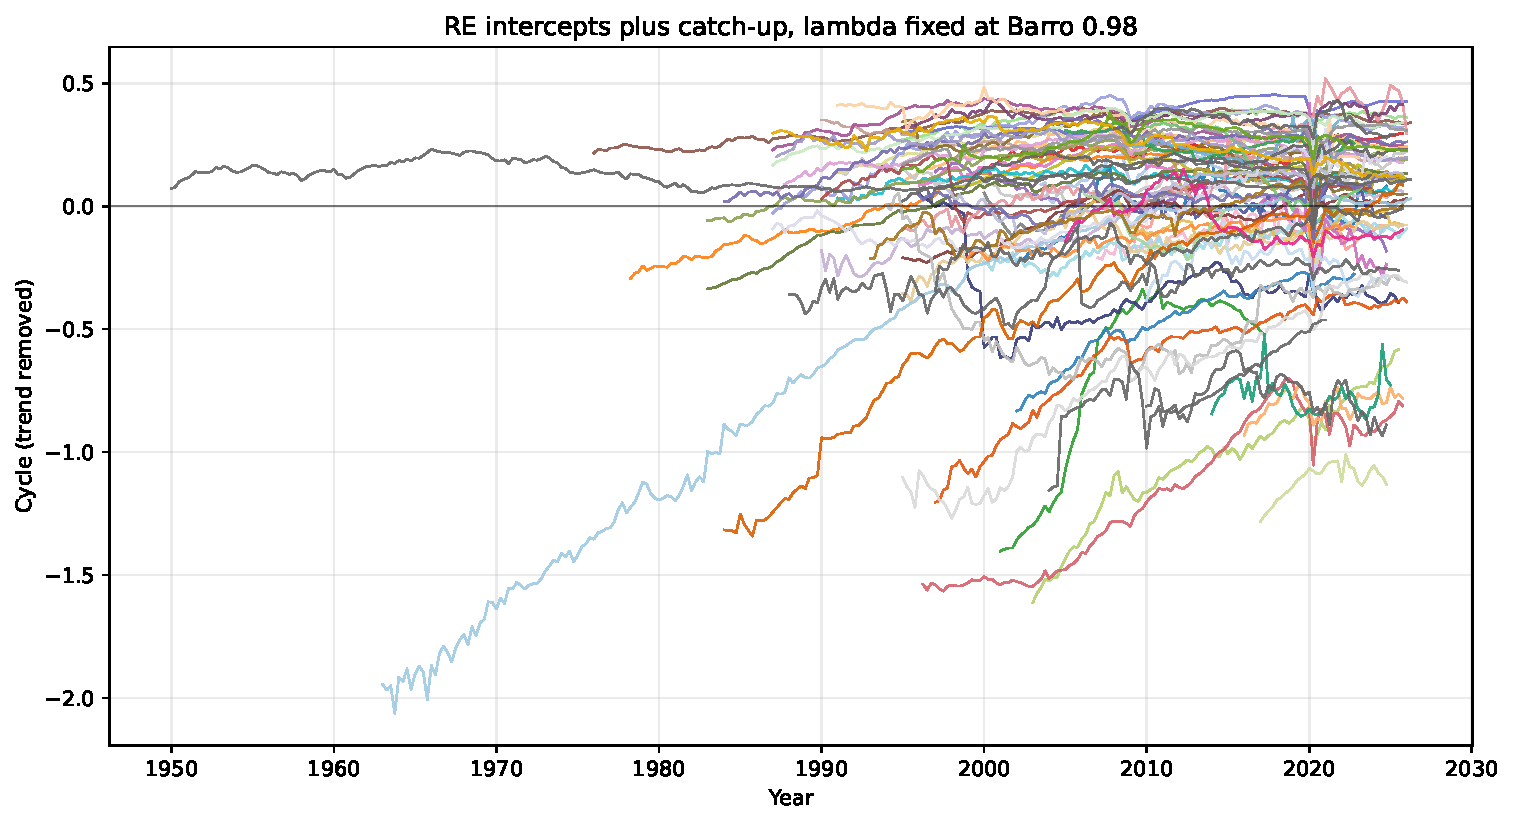
\includegraphics[width=0.75\textwidth]{figs/cycle_lambda_barro.pdf}
\caption{Country cycles after removing $a_i + g t + b_i\lambda^{t-T_{i0}}$ (posterior-mean $a_i$, $b_i$).}
\end{figure}
\clearpage
\section{RE intercepts plus catch-up, free lambda in (0, 0.985)}
2026-09-17 SA panel, full sample: log real GDP per worker. 74 countries, 8670 observations, 1950-Q1--2026-Q2. Fitted countries: 74. Observations: 8670. Log-likelihood: 23584.47. Ergodic mean of the cycle $E[z]=0.0236$ (0.0296).
Permanent RE intercepts and catch-up $y_{it}=a_i + g t + b_i\lambda^{t-T_{i0}}+z_{it}$ with $\alpha=-5.3357$ (0.0470), $\omega=0.7218$ (0.0084), $\lambda=0.9836$ (0.0014), $\omega_b=0.4311$ (0.0166). Posterior-mean $a_i$: mean -5.464, min -8.013, max -3.627. Posterior-mean $b_i$: mean -0.128, min -1.016, max 1.020. Common slope $g=0.0089$ (0.0005).
\begin{table}[h]
\centering
\caption{Regime AR(1), transition matrix, and ergodic $\pi$. Columns are regimes.}
\begin{tabular}{lccc}
\toprule
 & (0) & (1) & (2) \\
\midrule
$\mu$ & -0.9498 & 0.0000 & 0.2469 \\
 & (0.1280) & --- & (0.0357) \\ \addlinespace
$\sigma$ & 0.0740 & 0.0182 & 0.0068 \\
 & (0.0027) & (0.0005) & (0.0002) \\ \addlinespace
$\rho$ & 0.9896 & 0.9899 & 0.9900 \\
 & (0.0014) & (0.0002) & (0.0000) \\ \addlinespace
$\Pi_{0\cdot}$ & 0.6927 & 0.2953 & 0.0120 \\
 & (0.0342) & (0.0353) & (0.0076) \\ \addlinespace
$\Pi_{1\cdot}$ & 0.0632 & 0.8803 & 0.0565 \\
 & (0.0091) & (0.0122) & (0.0067) \\ \addlinespace
$\Pi_{2\cdot}$ & 0.0033 & 0.0508 & 0.9459 \\
 & (0.0047) & (0.0082) & (0.0056) \\ \addlinespace
$\pi$ & 0.0940 & 0.4327 & 0.4732 \\
 & (0.0101) & (0.0216) & (0.0257) \\ \addlinespace
\bottomrule
\end{tabular}
\end{table}
\begin{figure}[h]
\centering
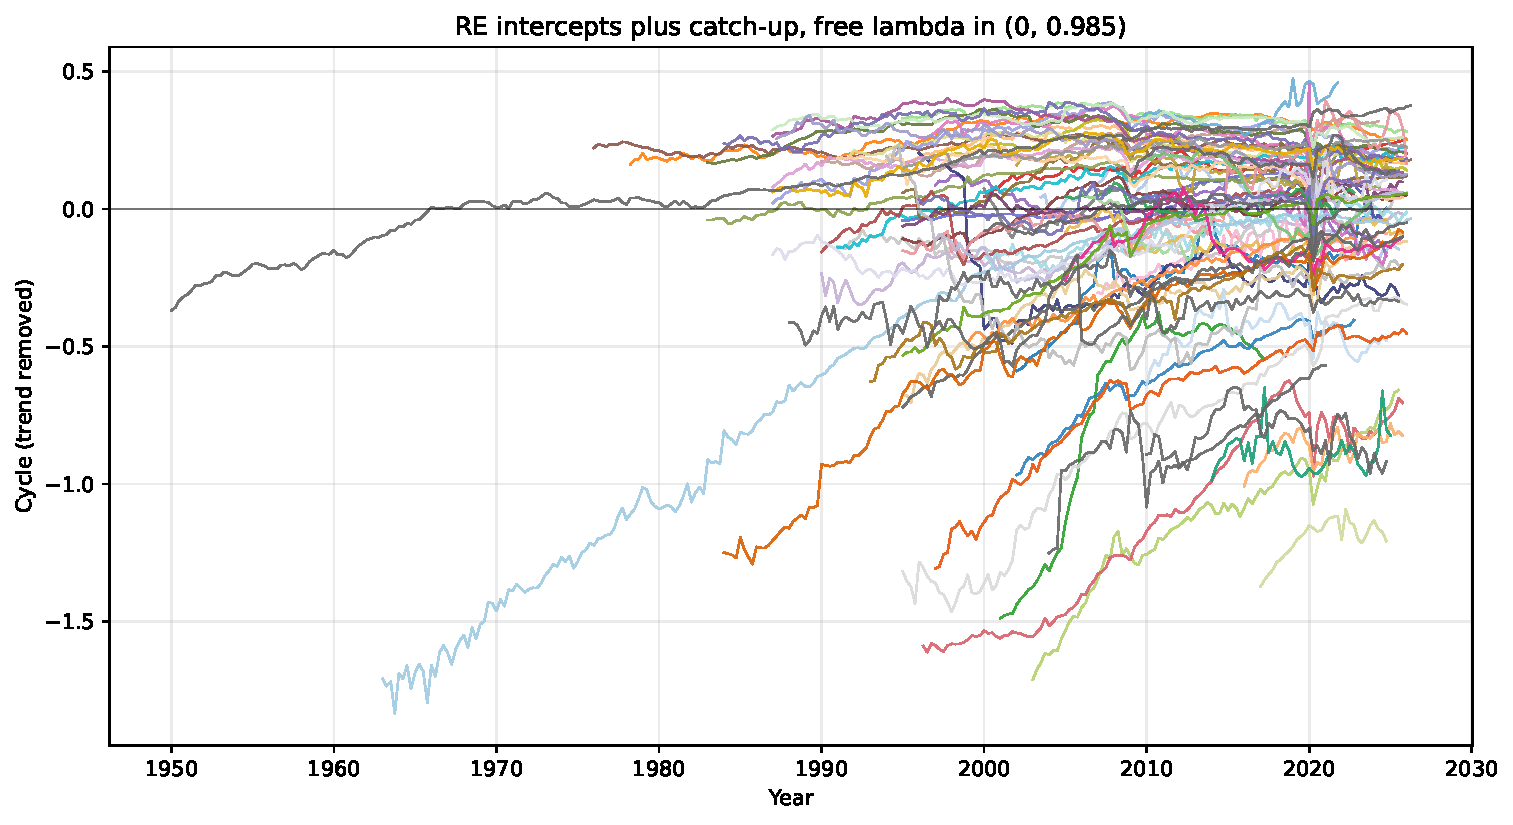
\includegraphics[width=0.75\textwidth]{figs/cycle_lambda_free.pdf}
\caption{Country cycles after removing the deterministic path.}
\end{figure}
\end{document}
